\documentclass{article}
\usepackage[utf8]{inputenc}
\usepackage[T1]{fontenc}
\usepackage{lmodern}
\usepackage[english]{babel}
\usepackage{amsmath, amssymb, amsthm, stmaryrd}
\usepackage{tikz}

\newcommand{\G}{\mathbb{G}}

\newtheorem{theorem}{Theorem}

\title{Extending results for an arbitrary set of generations}
\author{}

\begin{document}

\maketitle

\section{Notations}

We denote by $\G$ the set of generations, and $Y$ the set of utility values.\\
The set of utility streams is $X=Y^\G$.\\
$\kappa$ is a non-empty family of subsets of $\G$, stable by union and which doesn't
contain $\emptyset$.\\
$\mu$ is a subgroup of $\mathfrak{S}_\G$.

\section{Axioms}

We define the $\kappa$-relation as:
\[<_\kappa = \{(x,y)\in X^2|\forall i\in \G, x_i \leq y_i \land
\{j \in \G | x_j < y_j\}\in\kappa\}\]
$<_\kappa$ is a strict order:
\begin{itemize}
  \item Irreflexive since $\emptyset\not\in\kappa$.
  \item Asymmetric because $x<_\kappa y$ implies that for all $i\in\G$,
        $x_i\leq y_i$, and there exists $j$ such that $x_j < y_j$. Hence
        it is not possible to have $x<_\kappa y$ and $y<_\kappa x$.
  \item Transitive since $\kappa$ is stable by union.
\end{itemize}
We note $\leq_\kappa$ the reflexive closure of $<_\kappa$.\smallskip\par

\textbf{$\kappa$-Pareto}:
\[\forall x,y\in X, x <_\kappa y \Rightarrow x \prec y\]

\textbf{$\mu$-anonymity}:
\[\forall\sigma\in\mu,\forall x\in X, x \sim \sigma x\]

These two axioms can be extended as usual over social welfare functions.

\section{Grading principle}
\ \par
\textbf{$\kappa$-$\mu$ grading principle}:
\[\precsim_{\kappa\mu} = \{(x,y)\in X^2 |
\exists\sigma\in\mu, x \leq_\kappa \sigma y\}\]

Adaptation of theorem 1 in \cite{svensson80}:
\begin{theorem}
    $\precsim_{\kappa\mu}$ is a $\mu$-anonymous quasi-ordering on $X$, and
    $\kappa$-paretian if...
\end{theorem}
\begin{proof}
    \textbf{Reflexivity}: we can take $\sigma = Id\in\mu$ since $\mu$ is a
    subgroup of $\mathfrak{S}_\G$.\\
    \textbf{Transitivity}: if $x,y,z\in X$ such that $x \precsim_{\kappa\mu} y$ and 
    $y \precsim_{\kappa\mu} z$,
    we take $\sigma,\sigma'\in \mu$ such that $x\leq_\kappa \sigma y$ and
    $y\leq_\kappa \sigma' z$. We have $x\leq_\kappa (\sigma\circ\sigma')z$,
    and $\sigma\circ\sigma'\in\mu$ since $\sigma$ and $\sigma'$ are both in $\mu$.\\
    \textbf{$\mu$-anonymity}: if $x\in X$ and $\sigma\in\mu$, then
    $x\leq_\kappa\sigma^{-1}\sigma x$ with $\sigma^{-1}\in\mu$,
    therefore $x \precsim_{\kappa,\mu} \sigma x$. On the other hand,
    $\sigma x \leq_{\kappa}\sigma x$, hence $x \sim_{\kappa, \mu}\sigma x$.\\
    \textbf{$\kappa$-Pareto}: if we have $x,y\in X$ with $x<_\kappa y$, is there a
    $\sigma\in \mu\mathfrak{S}_\G$ such that $y\leq_\kappa \sigma x$? 
\end{proof}

\section{Existence of SWF}

Adaptation of theorem 1 of \cite{basumitra03}:
\begin{theorem}
  There is no SWF satisfying $\kappa$-Pareto and $\mu$-anonymity axioms if $\kappa$
  contains a subset $k$ of $\mathbb G$ such that $\mathbb G\setminus k$ is infinite,
  $|\mathbb G\setminus k|\geq |k|$ and $\mu$ contains the permutations of size $|k|$.
\end{theorem}

Recall of the proof in \cite{basumitra03} : we say that $0$ and $1$ are in $Y$ and
create for each real $0<z<1$ two utility streams $a(z)$ and $b(z)$ in
$\{0,1\}^{\mathbb N}$ such that $b(z)$ is bigger than $a(z)$ by only one bit and
that $a(z')$ is bigger than $a(z)$ by infinitely many bits when $z'>z$, so that we
can swap 2 bits to compare $b(z')$ to $a(z)$ to say it is smaller and that all the
$[W(a(z)),W(b(z))]$ are disjoint and non empty.

\begin{proof}
  We assume that $Y$ contains at least two elements that we identify wlog. to $0$
  and $1$ (else there is only one possible utility stream).

  Let:
  \begin{itemize}
  \item $k\in\kappa$ satisfying the conditions
  \item $s$ be a bijection of $G\setminus k$ in $(G\setminus k)\times
        (\mathbb Q\,\cap\,]0,1[)$
  \item $\pi_2$ be the projection of $(G\setminus k)\times (\mathbb Q\,\cap\,]0,1[)$
        in $\mathbb Q\,\cap\,]0,1[$
  \item $f=\pi_2\circ s:\mathbb G\setminus k\to\mathbb Q\,\cap\,]0,1[$
  \item $E(z)=\{g\in \mathbb G\setminus k\,|\, f(g)<z\}$ for $0<z<1$
  \item $\displaystyle a(z)=\left(\left\{\begin{array}{ll}1&\text{if }g\in
        E(z)\\0&\text{else}\end{array}\right.\right)_{g\in\mathbb G}$ for $0<z<1$
  \item $\displaystyle b(z)=\left(\left\{\begin{array}{ll}1&\text{if }g\in
        k\\a(z)&\text{else}\end{array}\right.\right)_{g\in\mathbb G}$ for $0<z<1$.
  \end{itemize}

  Therefore $\forall g\in k, a(z)_g=0$ and $b(z)_g=1$, so $a(z)<_\kappa b(z)$.

  \begin{center}
    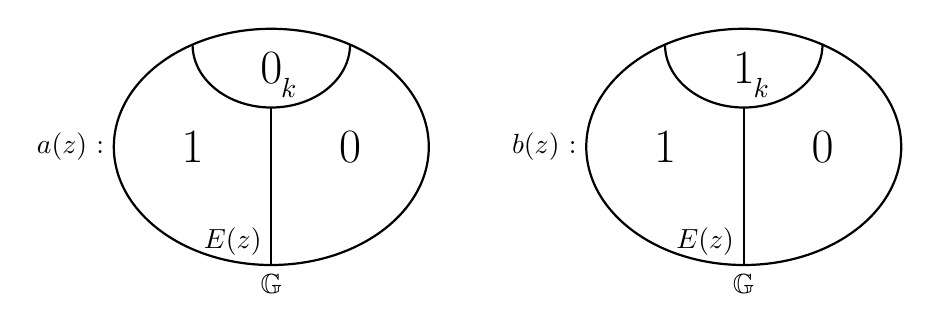
\begin{tikzpicture}
      \foreach \x/\lettre/\dansk in {0/a/0, 6/b/1} {
        \node[left]       (\lettre) at (\x-2,0) {$\lettre(z)$ :};
        \draw[thick]      (\x,0) ellipse (2 and 1.5);
        \node[below]      (G\x) at (\x,-1.5) {$\mathbb G$};
        \draw[thick]      (\x-1,1.3) arc (-180:0:1 and 0.8);
        \node[above right](k\x) at (\x,0.5) {$k$};
        \path[thick]      (\x,0.5) edge (\x,-1.5);
        \node[above left] (Ez\x) at (\x,-1.5) {$E(z)$};
        \node             (1\x) at (\x-1,0) {\LARGE{1}};
        \node             (0\x) at (\x+1,0) {\LARGE{0}};
        \node             (\dansk\x) at (\x,1) {\LARGE{\dansk}};
      }
    \end{tikzpicture}
  \end{center}

  Let $0<z<z'<1$.

  We want to show that $W(b(z))<W(a(z'))$.

  \begin{center}
    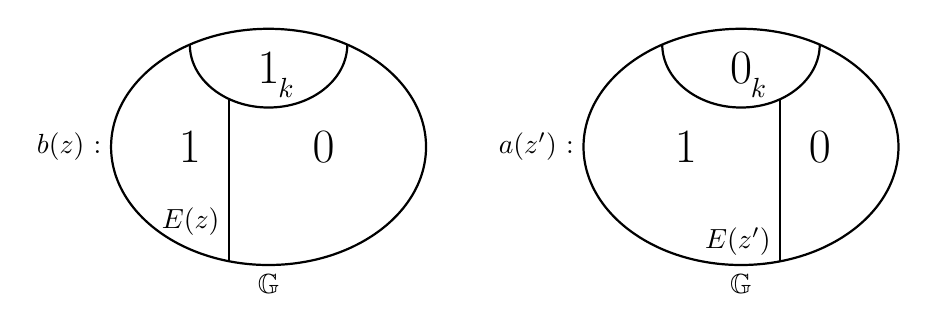
\begin{tikzpicture}
      % b(z)
      \node[left]       (bz) at (0-2,0) {$b(z)$ :};
      \draw[thick]      (0,0) ellipse (2 and 1.5);
      \node[below]      (G0) at (0,-1.5) {$\mathbb G$};
      \draw[thick]      (0-1,1.3) arc (-180:0:1 and 0.8);
      \node[above right](k0) at (0,0.5) {$k$};
      \path[thick]      (-0.5,0.6) edge (-0.5,-1.45);
      \node[above left] (Ez0) at (-0.5,-1.25) {$E(z)$};
      \node             (1b) at (-1,0) {\LARGE{1}};
      \node             (0b) at (0.7,0) {\LARGE{0}};
      \node             (1b) at (0,1) {\LARGE{1}};

      % a(z')
      \node[left]       (az) at (6-2,0) {$a(z')$ :};
      \draw[thick]      (6,0) ellipse (2 and 1.5);
      \node[below]      (G6) at (6,-1.5) {$\mathbb G$};
      \draw[thick]      (6-1,1.3) arc (-180:0:1 and 0.8);
      \node[above right](k6) at (6,0.5) {$k$};
      \path[thick]      (6.5,0.6) edge (6.5,-1.45);
      \node[above left] (Ez6) at (6.5,-1.5) {$E(z')$};
      \node             (16) at (6-0.7,0) {\LARGE{1}};
      \node             (06) at (6+1,0) {\LARGE{0}};
      \node             (06) at (6,1) {\LARGE{0}};
    \end{tikzpicture}
  \end{center}

  We are going to create two permutation $\sigma_1,\sigma_2\in\mu$ such as
  $\sigma_1 b(z)<_\kappa \sigma_2 a(z')$:

  \begin{center}
    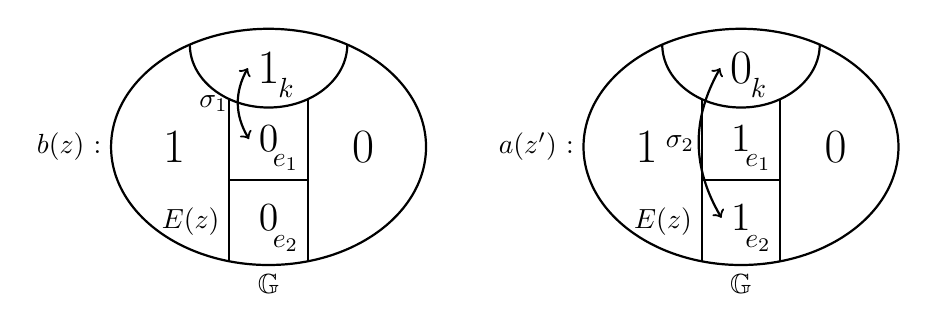
\begin{tikzpicture}
      \foreach \x/\noeud/\k/\e/\s in {0/b(z)/1/0/1, 6/a(z')/0/1/2} {
        \node[left]       (bz) at (\x-2,0) {$\noeud$ :};
        \draw[thick]      (\x,0) ellipse (2 and 1.5);
        \node[below]      (G0) at (\x,-1.5) {$\mathbb G$};
        \draw[thick]      (\x-1,1.3) arc (-180:0:1 and 0.8);
        \node[above right](k0) at (\x,0.5) {$k$};
        \path[thick]      (\x-.5,0.6) edge (\x-.5,-1.45);
        \path[thick]      (\x+0.5,0.6) edge (\x+0.5,-1.45);
        \path[thick]      (\x+0.5,-0.425) edge (\x-.5,-0.425);
        \node[above left] (Ez) at (\x-0.5,-1.25) {$E(z)$};        \node[above left] (e1) at (\x+.5,-0.425) {$e_1$};
        \node[above left] (e2) at (\x+.5,-1.45) {$e_2$};
        \node             (1Ez) at (\x-1.2,0) {\LARGE{1}};
        \node             (0G) at (\x+1.2,0) {\LARGE{0}};
        \node             (e1) at (\x,0.1) {\Large{\e}};
        \node             (e2) at (\x,-0.9) {\Large{\e}};
        \node             (k) at (\x,1) {\LARGE{\k}};
        \path[<->, thick] (e\s.west) edge [bend left] node[left=-2*\e] {$\sigma_{\s}$} (k.west);
      }
    \end{tikzpicture}
  \end{center}

  Since there is a rational $z<r<z'$,
  \[\forall g\in \mathbb G\setminus k, \pi_2(g,r)\in]z,z'[,\]
  so $|\pi_2^{-1}(]z,z'[)|\geq|G\setminus k|$. And because $s$ is a bijection,
  \[|\pi_2^{-1}(]z,z'[)|=|s^{-1}(\pi_2^{-1}(]z,z'[))|= |f^{-1}(]z,z'[)|.\]

  Therefore $|E(z')\setminus E(z)|\geq|G\setminus k|\geq |k|$, then because
  $E(z')\setminus E(z)$ is infinite we can divide it in two sets $e_1$ and
  $e_2$ of same cardinality. Then there are two injections $\iota_i$ from $k$ to
  $e_i$. Define $\sigma_i$ as $\underset{g\in k}{\text{\LARGE $\circ$}}
  \tau(g,(\iota_i(g))$.

  \begin{center}
    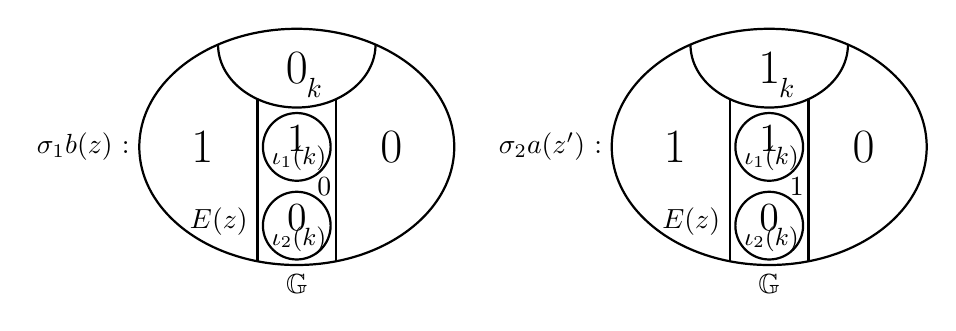
\begin{tikzpicture}[scale=1]
      \foreach \x/\noeud/\k in {0/\sigma_1b(z)/0, 6/\sigma_2a(z')/1} {
        \node[left]       (bz) at (\x-2,0) {$\noeud$ :};
        \draw[thick]      (\x,0) ellipse (2 and 1.5);
        \node[below]      (G0) at (\x,-1.5) {$\mathbb G$};
        \draw[thick]      (\x-1,1.3) arc (-180:0:1 and 0.8);
        \node[above right](k0) at (\x,0.5) {$k$};
        \path[thick]      (\x-.5,0.6) edge (\x-.5,-1.45);
        \path[thick]      (\x+0.5,0.6) edge (\x+0.5,-1.45);
        %\path[thick]      (\x+0.5,-0.425) edge (\x-.5,-0.425);
        \node[above left] (Ez) at (\x-0.5,-1.25) {$E(z)$};
        \node[above left] (te1) at (\x+.5,-0.425) {\small{$\iota_1(k)$}};
        \node[above left] (te2) at (\x+.5,-1.45) {\small{$\iota_2(k)$}};
        \node             (1) at (\x-1.2,0) {\LARGE{1}};
        \node             (0) at (\x+1.2,0) {\LARGE{0}};
        \node             (1) at (\x,0.1) {\Large{1}};
        \node             (0) at (\x,-0.9) {\Large{0}};
        \draw[thick]      (\x, 0) circle (0.43);
        \draw[thick]      (\x, -1) circle (0.43);
        \node             (1) at (\x,1) {\LARGE{\k}};
        \node             (1) at (\x+0.35,-0.5) {\k};
      }
    \end{tikzpicture}
  \end{center}

  Let $g\in\mathbb G$.

  If $g\in k$ then
  \[(\sigma_1 b(z))_g=b(z)_{\underset{\notin E(z)\cup k}
  {\underbrace{\sigma_1^{-1}(g)}}}=0<1=(\sigma_2 a(z'))_g=
  a(z')_{\underset{\in e_2}{\underbrace{\sigma_2^{-1}(g)}}}.\]

  If $g\in \iota_1(k)$ then
  \[(\sigma_1 b(z))_g=b(z)_{\underset{\in k}{\underbrace{\sigma_1^{-1}(g)}}}=
  1=(\sigma_2 a(z'))_g=a(z')_{\underset{=g\in e_1}
  {\underbrace{\sigma_2^{-1}(g)}}}.\]

  If $g\in \iota_2(k)$ then
  \[(\sigma_1 b(z))_g=b(z)_{\underset{=g \notin E(z)\cup k}
  {\underbrace{\sigma_1^{-1}(g)}}}=0=(\sigma_2 a(z'))_g=a(z')_{\underset{\in k}
  {\underbrace{\sigma_2^{-1}(g)}}}.\]

  Else
  \[(\sigma_1 b(z))_g=a(z)_g\leq (\sigma_2 a(z'))_g=a(z')_g.\] \\

  Hence $\sigma_1b(z)<_\kappa \sigma_2a(z')$, so by $\kappa$-Pareto
  $W(\sigma_1b(z))<W(\sigma_2a(z'))$.

  Furthermore, since $\sigma_1,\sigma_2\in\mu$, by $\mu$-anonymity we have
  $W(\sigma_1b(z))=W(b(z))$ and $W(\sigma_2a(z'))=W(a(z'))$.

  So $W(b(z))<W(a(z'))$, so $[W(a(z)),W(b(z))]$ and $[W(a(z')),W(b(z'))]$
  are disjoint and not reduced to one element (since $a(z)<_\kappa b(z)$), so to each real
  we can associate a unique and disjoint interval which is not a singleton. That is absurd because
  we could then associate a rational to each interval (by choosing one in the interval),
  thus those intervals would be countable.

\end{proof}



\bibliographystyle{alpha}
\bibliography{bibliography}
\end{document}
